\PassOptionsToPackage{usenames,dvipsnames,table,x11names}{xcolor}
\documentclass[8pt]{beamer}

% SETTING THEMES ----------------------------------------
%\usetheme{Warsaw}
\usetheme{Luebeck}
%\usetheme{Boadilla}

% COLORS IN PRESENTATION --------------------------------
\setbeamercolor*{palette primary}{bg = Firebrick1, fg = white}


%https://www.tug.org/pracjourn/2007-4/walden/color.pdf
%https://tex.stackexchange.com/questions/368784/change-color-in-beamer-theme

% FONT --------------------------------------------------
%\usefonttheme{professionalfonts} %doesn't do anything?
\usefonttheme{serif}

% CHANGING ITEMIZE ITEMS --------------------------------
\setbeamertemplate{itemize item}{\color{black} $\vcenter{\hbox{\tiny$\bullet$}}$} %style of item
\setbeamertemplate{itemize subitem}{\tiny \color{black}$\blacktriangleright$} %style for sub item
\setbeamercolor{itemize item}{fg=black} %changes color of all items

\setbeamertemplate{enumerate items}[default] %default number style
\setbeamercolor{enumerate item}{fg=black}

%\setbeamerfont{frametitle}{size=\Large}

%https://tex.stackexchange.com/questions/59742/progress-bar-for-latex-beamer

%\insertframenumber/\inserttotalframenumber

%getting rid of stuff on bottom
\setbeamertemplate{footline}[frame number]{}
\setbeamertemplate{navigation symbols}{}
%\setbeamertemplate{footline}{%
%    \raisebox{5pt}{\makebox[\paperwidth]{\hfill\makebox[20pt]{\color{gray}
%          \scriptsize\insertframenumber/\inserttotalframenumber}}}\hspace*{5pt}}

%\usepackage{natbib}
%\renewcommand\bibfont{\scriptsize}
\setbeamercolor*{bibliography entry title}{fg=black}
\setbeamercolor*{bibliography entry author}{fg=black}
\setbeamercolor*{bibliography entry location}{fg=black}

%\newcommand*{\myfont}{\fontfamily{phv}\selectfont} %helvecta
\newcommand*{\myfont}{\fontfamily{crm}\selectfont} %cm wont change
%https://tex.stackexchange.com/questions/25249/how-do-i-use-a-particular-font-for-a-small-section-of-text-in-my-document

%%%%%%%%%%%%%%%%%%%%%%%%%%%%%%%%%%%%%%%%%%%%%%%%%%%%%%%%%%
%%%%%%%%%%%%%%%%%%%%%%%%%%%%%%%%%%%%%%%%%%%%%%%%%%%%%%%%%%
%%%%%%%%%%%%%%%%%%%%%%%%%%%%%%%%%%%%%%%%%%%%%%%%%%%%%%%%%%

%------------------------------------------------------
%                Math Packages
%------------------------------------------------------

%\usepackage[intlimits]{amsmath}
\usepackage{amsmath}
\usepackage{amssymb}
\usepackage{amsthm}
%\everymath{\displaystyle}
\usepackage{siunitx} % for SI units (e.g. C, degree)
\usepackage{bm} % bold for some math symbols
\usepackage{nicefrac} % for nicer fractions sometimes
\usepackage[thinc]{esdiff} % for derivatives

%------------------------------------------------------
%                Tikz and Pgfplots
%------------------------------------------------------

\usepackage{pgfplots}
\usepackage{tkz-euclide}
\pgfplotsset{compat=1.15}
\usetikzlibrary{arrows,shadows,positioning, calc, decorations.markings, hobby, quotes,angles,decorations.pathreplacing,intersections, matrix,backgrounds}
\usepgfplotslibrary{polar,colormaps,fillbetween}
\usepgflibrary{shapes.geometric}
%\usetkzobj{all}

%------------------------------------------------------
%                Formatting
%------------------------------------------------------

% COLORS ----------------------------------------------
%\usepackage[dvipsnames, table]{xcolor}
\usepackage{xcolor}

% FIGURES ---------------------------------------------
\usepackage{graphicx} % for importing images
\usepackage{subcaption} % for making subfigures
\usepackage[labelfont=bf]{caption} % changing style of figures
% use font=it for italic font

% PAGE LAYOUT -----------------------------------------
%\linespread{1.3} % changes line spacing
\setlength{\parskip}{0.75em}

%\usepackage{indentfirst}
%\usepackage{parskip} % for not indenting paragraphs first
\usepackage{multirow} % having multiple rows
\usepackage{multicol} % having multiple columns
\usepackage[T1]{fontenc} % can combine \sc and \bf font

% LANGUAGES -------------------------------------------
\usepackage[english]{babel} % for correctly using english
\usepackage[utf8x]{inputenc} % compiling correctly
\usepackage{CJK} % using Chinese, Japanese, and Korean

% MISC ------------------------------------------------
\usepackage[normalem]{ulem} % for \sout
\usepackage{tikzsymbols} % for emojis
\usepackage{booktabs,eqparbox} % for tables
\usepackage{verbatim} % for verbatim environment
\usepackage{xmpmulti} % for animations

%------------------------------------------------------
%                Custom Commands
%------------------------------------------------------

\newcommand{\done}{\hfill $\square$ \vspace{1cm}}
\newcommand{\csch}{\mathrm{csch}}
\newcommand{\sech}{\mathrm{sech}}

%\newcommand{\dd}{\mathop{}\,\mathrm{d}}
\newcommand{\dd}{\;\mathrm{d}}

% COLOR CODING -----------------------------------------------
\newcommand{\code}[1]{\textcolor{Bittersweet}{\texttt{#1}}} % using for emphasizing variables, code, etc.
\newcommand{\mydef}[1]{\textcolor{SteelBlue3}{\textit{#1}}} % defining something

% VENN DIAGRAMS ----------------------------------------------
\def\firstcircle{(90:1.75cm) circle (2.5cm)}
\def\secondcircle{(210:1.75cm) circle (2.5cm)}
\def\thirdcircle{(330:1.75cm) circle (2.5cm)}
\def\sampspace{(-6,-4.25) rectangle (6,5)}  %Cartesian
%\def\sampspace{(225:7cm) rectangle (45:7cm)} %polar

% TO DO LIST -------------------------------------------------
%\usepackage{enumitem}

%\newlist{todolist}{itemize}{2}
%\setlist[todolist]{label=$\square$}

%\usepackage{pifont}
%\newcommand{\cmark}{\ding{51}}%
%\newcommand{\xmark}{\ding{55}}%
%\newcommand{\fin}{\rlap{$\square$}{\raisebox{2pt}{\color{Green}{\large\hspace{1pt}\cmark}}}%
%\hspace{-2.5pt}}
%\newcommand{\wontfix}{\rlap{$\square$}{\color{red}{\large\hspace{1pt}\xmark}}}

%------------------------------------------------------
%                Custom Environments
%------------------------------------------------------

\usepackage{mdframed}

% EXERCISE -------------------------------------------------
\mdfdefinestyle{exercise}{
	backgroundcolor=black!10,roundcorner=8pt,hidealllines=true,nobreak
}

%\begin{mdframed}[style=exercise]
%\end{mdframed}

% MATHEMATICA ------------------------------------------------
\mdfdefinestyle{mathematica}{
	backgroundcolor=Tan!15,roundcorner=8pt,hidealllines=true,nobreak,fontcolor=Bittersweet
}

% R ---------------------------------------------------------
\mdfdefinestyle{R}{
	backgroundcolor=SteelBlue3!15, roundcorner=8pt, hidealllines=true, nobreak, fontcolor=SteelBlue3
}

% R ---------------------------------------------------------
\mdfdefinestyle{python}{
	backgroundcolor=Green!15, roundcorner=8pt, hidealllines=true, nobreak, fontcolor=Green
}


\definecolor{Auburn}{rgb}{0.25, 0.1, 0}

%\usepackage[style=authoryear]{biblatex}

%%%%%%%%%%%%%%%%%%%%%%%%%%%%%%%%%%%%%%%%%%%%%%%%%%%%%%%%%%
%%%%%%%%%%%%%%%%%%%%%%%%%%%%%%%%%%%%%%%%%%%%%%%%%%%%%%%%%%
%%%%%%%%%%%%%%%%%%%%%%%%%%%%%%%%%%%%%%%%%%%%%%%%%%%%%%%%%%





\title{REU 2019 Presentation}
\author{Sparse Regression with Unsupervised Learning}
\institute{
\includegraphics[]{lamar_logo.jpeg}}
\date{Aiden Kenny, Danielle Solomon\\[0.5pt]
Lamar University\\[0.5pt]
\today}
    
\begin{document}

%%%%%%%%%%%%%%%%%%%%%%%%%%%%%%%%%%%%%%%%%%%%%%%%%%%%%%%%%%
%%%%%%%%%%% TITLE FRAME %%%%%%%%%%%
%%%%%%%%%%%%%%%%%%%%%%%%%%%%%%%%%%%%%%%%%%%%%%%%%%%%%%%%%%

\begin{frame}

\maketitle

\end{frame}

%%%%%%%%%%%%%%%%%%%%%%%%%%%%%%%%%%%%%%%%%%%%%%%%%%%%%%%%%%
%%%%%%%%%%% FRAME 1 %%%%%%%%%%%
%%%%%%%%%%%%%%%%%%%%%%%%%%%%%%%%%%%%%%%%%%%%%%%%%%%%%%%%%%

\begin{frame}{Introduction}

A \mydef{high-dimensional} data set is one where the number of predictors vastly outnumber the number of observations.
 
\begin{itemize}
    \item It presents several problems during analysis
    \vspace{4pt}
    \item It is difficult to take into account the influence of each of the predictors due to the exorbitant amount
    \vspace{4pt}
    \item Often times, predictors can be highly correlated.
    \vspace{4pt}
    \item From this large pool, some predictors are more influential than others.
    
\end{itemize}
\end{frame}
 
 
 
\begin{frame}{Goal}
   \textbf{We want to see if applying unsupervised clustering methods to data sets before employing supervised statistical learning techniques has the ability to improve prediction accuracy when classifying high-dimensional data.}
\end{frame}
 
 

\begin{frame}{Data}

A common real world occurrence of high-dimensional data is in gene expression data. 

Both data sets that we are working with are cancer gene expression data.

Genome data often has a group structure within the data set which is compatible with these particular regularization techniques. 

Both of these data sets have been previously used in studies for binary classification, specifically whether or not each gene is cancerous.

\end{frame}

\begin{frame}{Data}

COLON CANCER DATA (Alon et al)
\begin{itemize}
    \item 2000 genes chosen from a larger data set of 6500 genes (predictors)
    \item 62 tissues (observations) 
    \item binary classification (healthy vs tumor)
    \item 40 tumor tissues and 22 healthy tissues in the sample
    \item the genes with "the highest minimal intensity" across the 62 tissues
    \item The genes are placed in order of descending minimal intensity.
\end{itemize}

\noindent 
LEUKEMIA DATA
\begin{itemize}
    \item 72 patients (observations)
    \item 7128 genes (predictors)
    
\end{itemize}
\end{frame}



\begin{frame}{Statistical Models}

\mydef{Statistical learning} refers to various techniques used to understand data. 

\begin{itemize}
    \item When data is collected, it is stored in a \mydef{data matrix} $\mathbf{X}_{n \times p}$. 
\begin{itemize}
    \item Each row $\bm{x}_i$ of the matrix are the values for each observation. 
    \item Each column $\mathbf{x}_j$ of the matrix are the values of a predictor for all observations.
\end{itemize}
\end{itemize}

There is usually some response that is measured with each observation, and they are stored in the \mydef{response vector} $\mathbf{y}$. 

\begin{itemize}
\item Our goal is to fit a \mydef{statistical model} $f(\bm{x})$ that can use $\mathbf{X}$ to \mydef{predict} $\mathbf{y}$ 

\begin{itemize}
    \item These predictions are stored in a \mydef{prediction vector} $\hat{\mathbf{y}} = (f(\bm{x}_1), \ldots, f(\bm{x}_n))$. 
    \item This is known as \mydef{supervised learning}, where there is a response that can be measured.
\end{itemize}
\end{itemize} 

There are two goals for a statistical model: 
\begin{enumerate}
    \item \mydef{Prediction}: want predictions $\hat{\mathbf{y}}$ to be accurate.
    \item \mydef{Interpretation}: want to know which predictors are important in determining the response.
\end{enumerate}
\end{frame}


 
\begin{frame}{Flexibility and the Bias-Variance Trade-Off}

Loosely speaking, a statistical learning method is \mydef{flexible} if it is able to fit a wide variety of forms for $f(\bm{x})$. 
\begin{itemize}
    \item The more flexible a model becomes, the more parameters that need to be estimated.
    \item The more flexible a model is, the less interpretable. 
    \item If model is too flexible, it will also over-fit. 
\end{itemize}

There are two main characteristics of a statistical model: 
\begin{enumerate}
    \item \mydef{Bias}: the error introduced by estimating a more complicated model with a simpler model. 
    \item \mydef{Variance}: how much the model would change if it were fit using a different training set. 
\end{enumerate}

As a model becomes more flexible, its bias will \textit{decrease} while its variance will \textit{increase} 

There is a flexibility ``sweet-spot'' where both the bias and variance are low enough to have the lowest test error; this is known as the \mydef{bias-variance trade-off}.
    
\end{frame}


\begin{frame}{Supervised  Statistical Models}
We have two types of supervised statistical models: 
\begin{enumerate}
    \item \mydef{Regression models}: the response is continuous (we will focus on this one). 
    \item \mydef{Classification models}: the response is categorical.
\end{enumerate}

How to determine prediction accuracy:
\begin{itemize}
    \item For regression, we can use the \mydef{mean-squared error}, $\displaystyle \mathrm{MSE} = \frac{1}{n} \| \mathbf{y} - \hat{\mathbf{y}} \|_2^2$. %\pause
    \item For classification, we can use the \mydef{error rate}, $\displaystyle \mathrm{ER} = \frac{1}{n} \sum_{i=1}^{n} \mathbb{I}(y_i \not= \hat{y}_i)$. %\pause
    \item The ideal error rate is the lowest one.
\end{itemize}

To avoid models from \mydef{over-fitting}: 
\begin{enumerate}
    \item Randomly divide the data into a training set $\mathbf{X}_{\mathcal{R}}$ and a test set $\mathbf{X}_{\mathcal{T}}$. 
    
    \item We fit $f(\bm{x})$ using the test set $\mathbf{X}_{\mathcal{R}}$. 
    \item We check the prediction accuracy using the training set $\mathbf{X}_{\mathcal{T}}$. The best models will have the lowest \mydef{test error}.
\end{enumerate}
\end{frame}

\begin{frame}{Regularization}
\mydef{Regularization} is a useful technique when working with high-dimensional data sets.

\begin{itemize}   
    \item It aims to introduce a small amount of bias in the model with the hopes of drastically lowering the variance, thus improving prediction accuracy in classification.
    
     \item Various regression models (e.g. linear and logistic) can be modified by many kinds of penalties which allow different types of regularization to occur.
\end{itemize}
\end{frame}





\begin{frame}{Logistic Regression}
\begin{itemize}
    \item Many classification problems are \mydef{binary}, meaning the response falls into two classes. 
    
    \item For convenience, the response will be coded as $Y \in \{ 0,1 \}$.
    
    \item We wish to model the \mydef{probability} that the response falls into either class, given an input $X$. 
    
    \item Let $p(\bm{x}) = \mathbb{P}(Y = 1 \mid X = \bm{x})$, and so $1 - p(\bm{x}) = \mathbb{P}(Y = 0 \mid X = \bm{x})$. The response $\mathbf{y} = (y_1, \ldots, y_n)$ is modeled as 
    \begin{align*}
    \log \left( \frac{p(\bm{x}_i)}{1 - p(\bm{x}_i)} \right) = \beta_0 + \bm{x}_i^T \bm{\beta}, \\
    y_i = \begin{cases}
        1 & \text{if } p(\bm{x}_i) \ge 0.5 \\
        0 & \text{if } p(\bm{x}_i) < 0.5
    \end{cases}.
    \end{align*}

\end{itemize}
\end{frame}



\begin{frame}{Logistic Regression}

or alternatively, 
    \begin{align*}
    p(\bm{x}_i) = \frac{e^{\beta_0 + \bm{x}_i^T \bm{\beta}}}{1 + e^{\beta_0 + \bm{x}_i^T \bm{\beta}}}.
    \end{align*}
Here, $\beta_0$ and $\bm{\beta} = (\beta_1, \ldots, \beta_p)$ must be estimated from the data. This is done by minimizing the \mydef{negative log-likelihood function}, given by 
\begin{align}
\label{negloglike}
    \mathcal{L}(\beta_0, \bm{\beta}) = - \frac{1}{n} \sum_{i = 1}^n \Big[ y_i\big(\beta_0 + \bm{x}_i^T \bm{\beta}\big) - \log \left(1 + e^{\beta_0 + \bm{x}_i^T \bm{\beta}}  \right) \Big]. 
\end{align}

$\mathcal{L}(\beta_0, \bm{\beta})$ is convex, so it can be optimized efficiently.

\end{frame}



\begin{frame}{Logistic Regression}
\begin{itemize}
    \item We also will consider fitting the logistic regression model in the group setting. 
    
    \item This was introduced in \cite{meier2008group}. Suppose now that the predictors in the data matrix $\mathbf{X}$ are split up into $K$ groups.  
    
    \item Assume that the groups are non-overlapping. 
    
    \item Let $p_k$ denote the number of predictors in group $k$. 
    
    \item We have $p_1 + \ldots + p_k = p$ (the total number of predictors). 
    
    
\end{itemize}
\end{frame}

\begin{frame}{Logistic Regression}
\begin{itemize}
     \item Let $\bm{x}_{i,k} \in \mathbb{R}^{p_k}$ denote the vector having information about only the predictors in group $k$. So 
    
\begin{align*}
    \bm{x}_{i,k} = \begin{pmatrix}
        x_{i,1} \\ \vdots \\ x_{i, p_k}
        \end{pmatrix}
\end{align*}

and

\begin{align*}
    \bm{x}_i = \begin{pmatrix}
    \bm{x}_{i,1}^T & \cdots & \bm{x}_{i,K}^T
    \end{pmatrix}.
\end{align*}

    \item In other words, we are re-writing $\bm{x}_i$ as a vector whose elements are vectors. 
\end{itemize}
\end{frame}


\begin{frame}{Logistic Regression}
\begin{itemize}
    \item More generally, let $\mathbf{X}_k \in \mathbb{R}^{n \times p_k}$ is the matrix whose columns are the predictors in group $k$. So 

\begin{align*}
    \mathbf{X}_k = \begin{pmatrix}
    \bm{x}_{1,k}^T \\
    \vdots \\
    \bm{x}_{n,k}^T
    \end{pmatrix}
\end{align*}

and 

\begin{align*}
\mathbf{X} = \begin{pmatrix}
\mathbf{X}_1 & \cdots & \mathbf{X}_K
\end{pmatrix} = \begin{pmatrix}
\bm{x}_{1,1}^T & \cdots & \bm{x}_{1,K}^T \\
\vdots & \ddots & \vdots \\
\bm{x}_{n,1}^T & \cdots & \bm{x}_{n,K}^T
\end{pmatrix}.
\end{align*}

\end{itemize}
\end{frame}

\begin{frame}{Logistic Regression}
\begin{itemize}
    \item Let $\bm{\beta}_k \in \mathbb{R}^{p_k}$ be the sub vector of $\bm{\beta}$ corresponding to group $k$. 
    \item The goal here is to model $p(\bm{x}_i)$ using the \textit{groups}, $\bm{x}_{i,k}$
    \item The logistic regression model in the group setting now takes the form 
    
\begin{align}
    \label{logreggroup}
        \log \left( \frac{p(\bm{x}_i)}{1 - p(\bm{x}_i)} \right) = \beta_0 + \sum_{k=1}^K \bm{x}_{i,k}^T \bm{\beta}_k \triangleq \eta_K(\bm{x}_i).
\end{align}

    \item Now the coefficients are estimating by minimizing the negative log-likelihood function, which now becomes 
    
\begin{align}
    \label{negloglikegroup}
        \mathcal{L}_K(\beta_0, \bm{\beta}) = - \frac{1}{n} \sum_{i = 1}^n \Big[ y_i\big(\eta_K(\bm{x}_i)\big) - \log \big(1 + e^{\eta_K(\bm{x}_i)}  \big) \Big].
\end{align}

\end{itemize}
\end{frame}





\begin{frame}{Regularization}

\begin{itemize}
    \item Regularization (a.k.a. \mydef{shrinkage}) involves shrinking the estimated coefficients $\hat{\bm{\beta}}$ toward zero. 
\begin{itemize}
    \item The goal is to have a \textit{small} increase in bias to give a \textit{large} decrease in variance. 
    \item There are various shrinkage estimation techniques. 
\end{itemize}

    \item There are some things that are standard to all regularization techniques: 
\begin{itemize}
    \item We always \mydef{center} the data, such that the average value for each predictor $\mathbf{x}_j$ is zero. 
    \item As a result, the intercept coefficient is estimated by $\displaystyle \hat{\beta}_0 = \frac{1}{n} \sum_{i=1}^n y_i$. So we are only shrinking $\bm{\beta} = (\beta_1,\ldots,\beta_p)$. 
\end{itemize}

    \item These can be applied to a wide variety of models, but this presentation will focus on linear regression.

\end{itemize}  
\end{frame}

\begin{frame}{Ridge Regression}

\begin{itemize}
 
    \item \mydef{Ridge Regression} \cite{hoerl1970ridge} shrinks the coefficients by imposing a \textit{squared} $\ell_2$ norm on $\bm{\beta}$. The estimates are found by minimizing the loss function
    
\begin{align*}
    J(\bm{\beta}) = \frac{1}{2} \| \mathbf{y}  - \mathbf{X} \bm{\beta} \|_2^2 + \lambda \| \bm{\beta} \|_2^2.
\end{align*} 

    \item $\lambda$ is a \mydef{tuning parameter} which affects the severity of the shrinkage (larger values correspond to more shrinkage). %\pause

    \item Can also be viewed as minimizing the loss function 
\begin{align*}
    J(\bm{\beta}) = \frac{1}{2} \| \mathbf{y}  - \mathbf{X} \bm{\beta} \|_2^2 ~~\text{ subject to }~~ \| \bm{\beta} \|_2^2 \le t,
\end{align*}

for some constant $t$. 

\begin{itemize}
    \item This constraint is known as the \mydef{shrinkage penalty}.
\end{itemize}

    \item The main drawback to ridge regression is that \textit{the estimated coefficients will almost never equal 0}. 
\begin{itemize}
    \item In other words, ridge regression results in \mydef{dense} models, since none of the predictors are left out. 
    \item May be okay for prediction, but bad for interpretability.
\end{itemize}

\end{itemize}

\end{frame}


\begin{frame}{Lasso}
\begin{itemize}
    \item \mydef{LASSO}, or Least Absolute Shrinkage and Selection Operator, is a regularization technique that shrinks the coefficient estimates to zero.

    \item Shrinking the coefficient estimates can significantly reduce variance. 
    
    \item The lasso coefficients, $\hat{\beta_{\lambda}^{L}}$, minimize the quantity 
    
    \begin{align}
    \label{lasso}
         \mathcal{L}(\beta_{0},\bm{\beta}) + \lambda \| \bm{\beta} \|_{1}.
    \end{align}
    
    \item The penalty is the $l_{1}$ norm $\|\beta\|_{1}$ = $\sum|\beta_{j}|$. 
    \item The $l_{1}$ penalty has the effect of forcing some of the coefficient estimates to be exactly equal to zero, when the tuning parameter $\lambda$ is sufficiently large.

\end{itemize}

\end{frame}

\begin{frame}{Lasso}

\begin{itemize}

    \item  Lasso yields \mydef{sparse models} - models that involve only a subset of the variables. 
    
    \item When $\lambda = 0$, lasso gives least squares regression fit.
    
    \item When $\lambda$ is sufficiently large, lasso gives the null model in which all coefficient estimates are equal to zero. 
    
    \item Another way to write lasso: we are minimizing $\mathcal{L}(\beta_0, \bm{\beta})$ subject to the constraint
   
    \begin{align*}
        \lambda \| \bm{\beta} \|_{1} \le \delta,
    \end{align*}
    
for some constant $\delta$. 

    \item The goal is to try to find the set of coefficient estimates that lead to the smallest RSS, subject to the constraint that there's a budget $s$  for how large $\| \bm{\beta} \|_1 =  \sum\limits_{j=1}\limits^{P} |\beta_{j}|$ can be.
    
    \item An extremely large $\delta$ gives budget that is not very restrictive, then coefficient estimates can be large.
    \item If $s$ is a small value, then $\sum\limits_{j=1}\limits^{p} |\beta_{j}|$ must be small to not violate the budget. 

\end{itemize}

\end{frame}

\begin{frame}{Lasso}
    Cross validation is used to choose the value for $\lambda$ (tuning parameter) or $s$ (constraint).
\begin{itemize}
     \item Choose a grid of $lambda$ values and compute the cross-validation error for each value.
     \item Select tuning parameter value for which the cross-validation error is the smallest. 
\end{itemize}
\end{frame}



\begin{frame}{Elastic Net}
\begin{itemize}
    \item Elastic net generalizes lasso and combines it with ridge regression by adding the $\ell_{2}$ penalty to the objective function of the lasso. 

    \item This method does not utilize the characteristic of being pre-clustered when dealing the predictors. 

    \begin{align*}
     \mathcal{L}(\beta_{0},\bm{\beta}) + \lambda_1 \| \bm{\beta} \|_{1} + \frac{\lambda_2}{2} \|\bm{\beta}\|_{2}^{2}.
    \end{align*}
    
    \item If $\lambda_1 = 0$, it behaves like ridge regression.
    
    \item If $\lambda_{2} = 0$, it behaves like lasso. Can alternatively be written as 

    \begin{align*}
         \mathcal{L}(\beta_0, \bm{\beta})
    + \lambda \Big[ \alpha \| \bm{\beta} \|_{1} + \frac{1 - \alpha}{2} \|\bm{\beta}\|_{2}^{2} \Big],
    \end{align*}
    
where $\alpha = \frac{\lambda_1}{\lambda_1 + \lambda_2}$ and $\lambda = \lambda_1 + \lambda_2$.

    \item $\alpha = 1$ corresponds to the lasso, while $\alpha = 0$ corresponds to ridge regression. $\alpha \in [0,1]$. 

\end{itemize}    
\end{frame}

\begin{frame}{Elastic Net}
\begin{itemize}
    \item This method is preferred, since it controls how much of a ridge and lasso penalty is applied. 
    \item Can make penalty ``more ridge'' or ``more lasso'' just by tuning $\alpha$. 
    \item Sometimes both $\hat{\lambda}$ and $\hat{\alpha}$ are estimated from cross validation. 
    \item However, it is also common to fit a model over a grid of $\alpha$ values and perform cross validation to determine $\lambda$ for each model.
\end{itemize}
\end{frame}

\begin{frame}{Contour Plots}

\begin{figure}
    \centering
    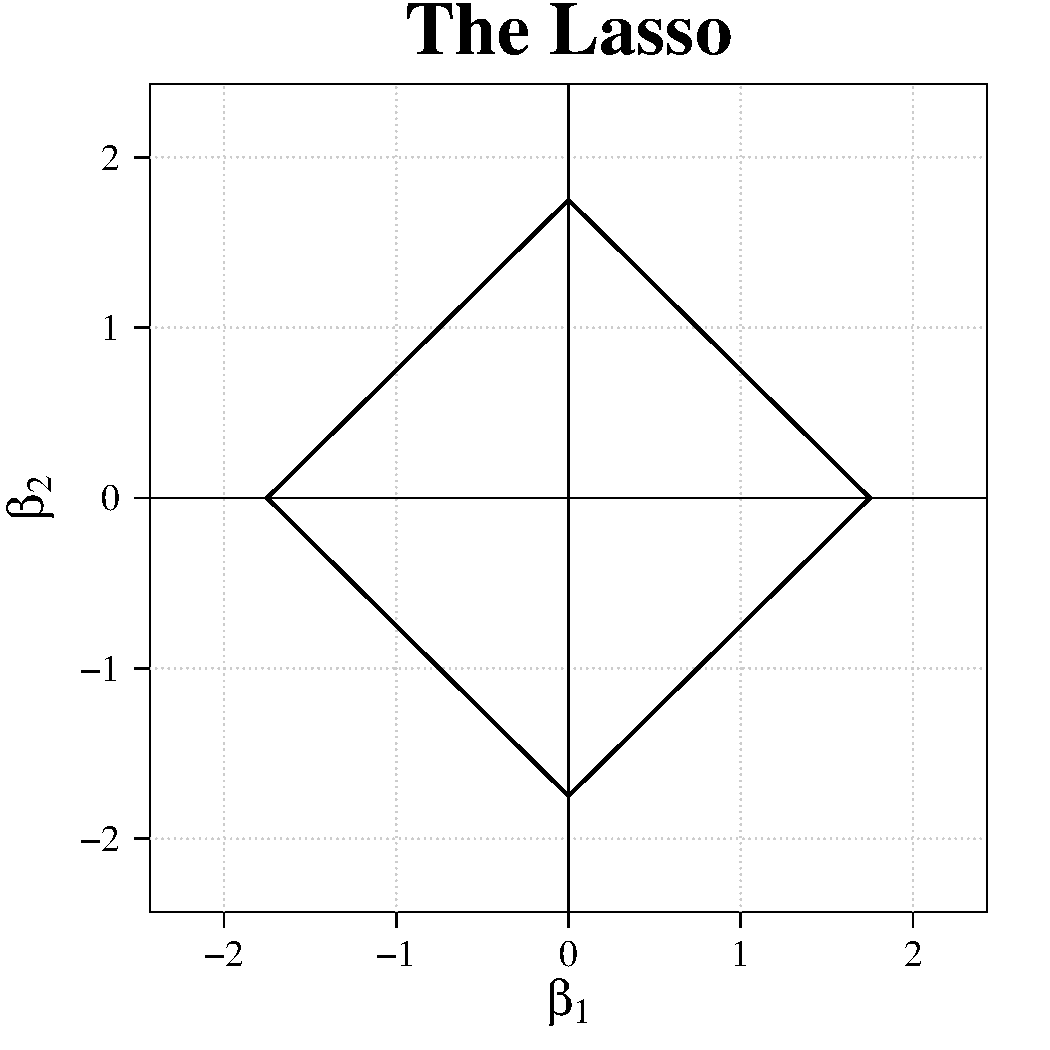
\includegraphics[width = 0.33\textwidth]{cont_lasso.pdf}
    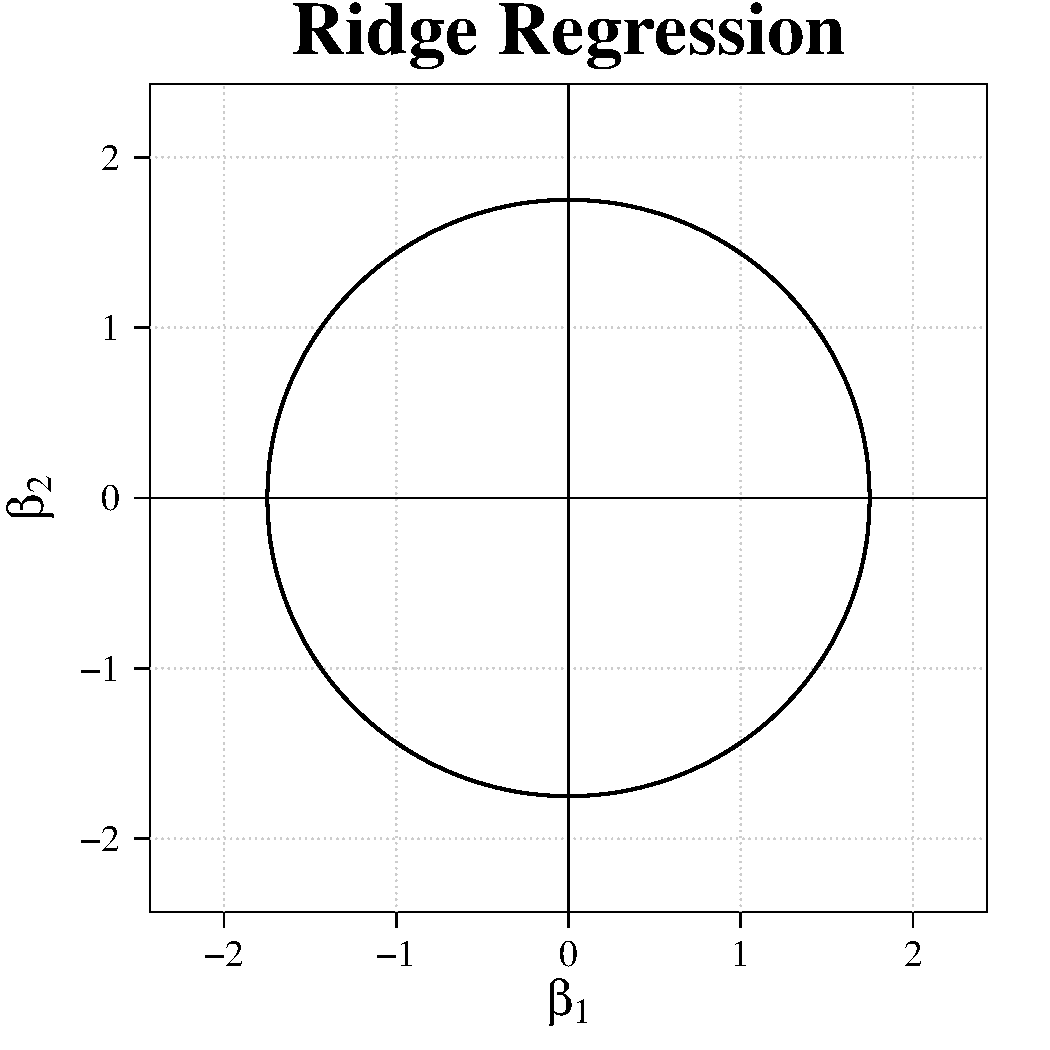
\includegraphics[width = 0.33\textwidth]{cont_ridge.pdf}
    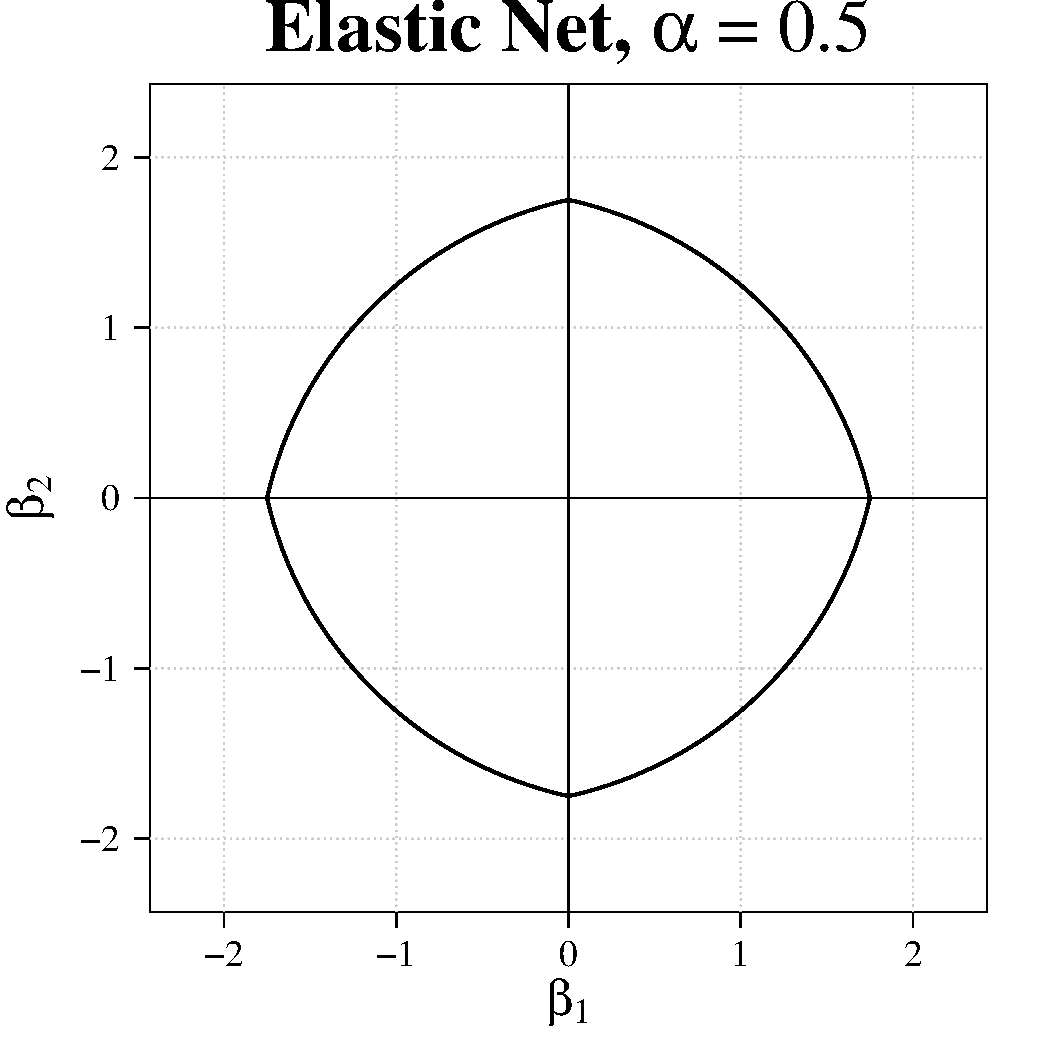
\includegraphics[width = 0.33\textwidth]{cont_enet.pdf}
    \caption{Contour plots for various regularization techniques for two predictors.}
    \label{mult_cont}
\end{figure} 

In the special case of two predictors, i.e. $\bm{\beta} = (\beta_1,\beta_2)$, the estimated coefficients $\hat{\bm{\beta}}$ will lie on the \mydef{contour line} of the shrinkage penalty. 

Gives some intuition about what type of shrinkage each method performs  

    
\end{frame}

\begin{frame}{The Group Setting}

When you have a data matrix $\mathbf{X}$, it is possible that each of the predictors belong to different \mydef{groups}. 

For example, let's say our data matrix $\mathbf{X}$ has $3$ observations and $6$ predictors, and is split up into four different groups. 
\begin{align*}
    \mathbf{X} &=
\begin{tikzpicture}[baseline=(m-2-1.base)]
        \matrix [matrix of math nodes,left delimiter=(,right delimiter=),
        ampersand replacement=\&] (m)
        {
            x_{1,1} \& x_{1,2} \& x_{1,3} \& x_{1,4} \& x_{1,5} \& x_{1,6} \\%[-1.5ex]               
            x_{2,1} \& x_{2,2} \& x_{2,3} \& x_{2,4} \& x_{2,5} \& x_{2,6} \\               
            x_{3,1} \& x_{3,2} \& x_{3,3} \& x_{3,4} \& x_{3,5} \& x_{3,6} \\           
        };  
        \begin{scope}[on background layer]
        \draw[color=Pink3, fill = Pink3, fill opacity = 0.25, rounded corners] (m-1-1.north west) -- (m-1-1.north east) -- (m-3-1.south east) -- (m-3-1.south west) -- cycle;
        \draw[color=SteelBlue3, fill = SteelBlue3, fill opacity = 0.25, rounded corners] (m-1-2.north west) -- (m-1-3.north east) -- (m-3-3.south east) -- (m-3-2.south west) -- cycle;
        \draw[color=orange, fill = orange, fill opacity = 0.25, rounded corners] (m-1-4.north west) -- (m-1-5.north east) -- (m-3-5.south east) -- (m-3-4.south west) -- cycle;
        \draw[color=Green4, fill = Green4, fill opacity = 0.25, rounded corners] (m-1-6.north west) -- (m-1-6.north east) -- (m-3-6.south east) -- (m-3-6.south west) -- cycle;
        \end{scope}
        \draw [decorate, decoration = {brace, amplitude = 5pt, mirror, raise = 2mm}, white] (m-3-1.south west) -- (m-3-1.south east) node[midway, yshift = -1em, align = center, black]{$\mathcal{G}_1$};
        \draw [decorate, decoration = {brace, amplitude = 5pt, mirror, raise = 2mm}, white] (m-3-2.south west) -- (m-3-3.south east) node[midway, yshift = -1em, align = center, black]{$\mathcal{G}_2$};
        \draw [decorate, decoration = {brace, amplitude = 5pt, mirror, raise = 2mm}, white] (m-3-4.south west) -- (m-3-5.south east) node[midway, yshift = -1em, align = center, black]{$\mathcal{G}_3$};
        \draw [decorate, decoration = {brace, amplitude = 5pt, mirror, raise = 2mm}, white] (m-3-6.south west) -- (m-3-6.south east) node[midway, yshift = -1em, align = center, black]{$\mathcal{G}_4$};
\end{tikzpicture}
\end{align*} %\pause

Note here that we have assumed that the groups do not \mydef{overlap}, so no predictor can be in two groups at once. %\pause

There are two ways to determine these groups: %\pause
\begin{enumerate}
    \item They are known to us from subject matter expertise. %\pause
    \item We can use various \mydef{clustering} techniques to determine them ourselves. %\pause
\end{enumerate}

We can use these groups to make predictions, as opposed to using the predictors individually.

\end{frame}

\begin{frame}{K-Means Clustering}

\begin{itemize}

\item \emph{K-means clustering} seeks to partition observations into a pre-specified number of clusters, so that observations within the groups are similar to each other, while observations in different groups are quite different from each other. 

\item \emph{K} is the pre-specified value of non-overlapping groups. 

\item Let $\mathcal{C} = \{ C_{1},..., C_{k} \}$ denote sets containing the indices of observations in each cluster. These sets satisfy two properties:

\begin{enumerate}
    \item $C_{1} \cup C_{2} \cup ... \cup C_{k} = \{1,\ldots,n\}$  (each observation belongs to at least one of $K$ clusters)
    
    \item $C_{k} \cap C_{k'} = \emptyset  $ for all $k \neq k'$ (no observation belongs to more than one cluster)
\end{enumerate}

\item If $i^{th}$ observation is in the $k^{th}$ cluster, $i \in C_{k}$.

\item A good clustering is one for which the within-cluster variation is as small as possible. 

\end{itemize}
\end{frame}

\begin{frame}{K-Means Clustering}

\begin{itemize}
\item Within-clustering variation ($W(C_{k})$): a measure of the amount by which the observations within a cluster differ from each other. 
\item \textit{Total Within-Cluster Variation}: the sum of all $W(C_k)$, and chooses the squared Euclidean distance as the dissimilarity measure.
    \begin{align}
     \label{kmeans}
      W(\mathcal{C}) = \sum_{k=1}^K W(C_k) = \sum_{k=1}^K \sum_{i \in C_k} \| \bm{x}_i - \bm{\mu}_k \|_2^2.
    \end{align}
\item $|C_{k}|$ denotes number of observations in the $k^{th}$ cluster. 
\item The within-cluster variation for the $k^{th}$ cluster is the sum of all pairwise squared Euclidean distances between the observations in the $k^{th}$ cluster, divided by the total number of observations in the $k^{th}$ cluster.
\item $K$-means clustering is a ``top-down'' method. We use the GAP statistic \cite{tibshirani2001estimating} to determine the number of clusters. These are both ``hard clustering'' methods, meaning the groups do not overlap. 
\end{itemize} 
\end{frame}

\begin{frame}{K-Means Clustering}
\begin{figure}
    \centering
    \includegraphics[width = 0.33\textwidth]{clus_2.pdf}
    \includegraphics[width = 0.33\textwidth]{clus_3.pdf}
    \includegraphics[width = 0.33\textwidth]{clus_4.pdf}
    \caption{Clustering the same data with varying numbers of clusters.}
    \label{mult_cluster}
\end{figure} %\pause

There are several methods to choose the amount of clusters: %\pause
\begin{itemize}
    \item We can just arbitrarily choose them. %\pause
    \item Use subject matter expertise. %\pause
    \item Several criterion functions exist, such as the \mydef{GAP statistic} \cite{tibshirani2001estimating}.
\end{itemize}
    
\end{frame}

\begin{frame}{Hierarchical Clustering}
\begin{itemize}
    \item \emph{Hierarchical clustering} provides an alternate method of clustering data. 
    \item Unlike $K$-means clustering, hierarchical clustering does not require pre-specified $k$ clusters.
    \item It results in a tree-based representation of the observations, known as a dendogram. A dendogram is constructed starting from the leaves and combining clusters up to the trunk. 
    \item Each leaf of the dendogram represents an observation. 
    \item When leaves begin to fuse into branches, it indicates that the observations are similar to each other. 
    \item Branches can fuse with other branches or leaves when moving further up the tree. 
    \item The height of the fusion indicates how similar or different the observations are. 
    \item Both $K$-means clustering and hierarchical clustering include all the observations in a data set.     
\end{itemize}   
\end{frame}

\begin{frame}{Group Lasso}

\begin{itemize}
    \item Predictors belong to predefined groups. 
    \item Group Lasso is used to shrink and select the members of a group together. 
    \item $p$ predictors are divided into $L$ groups, with $p_{l}$ being the number of groups in $l$
    \item matrix $\mathbf{X}_{l}$ represents predictors corresponding to the $l^{th}$ group, with corresponding coefficient vector $\beta_{l}$
    \item Group Lasso minimizes
    \[
    \min\limits_{\beta \in \mathbb{R}^{p}}
    (\|\mathbf{y}-\beta_{0}\mathbf{1}-\sum\limits_{l=1}\limits^{L}
    \mathbf{X}_{l}\beta_{l} \|_{2}^{2} + 
    \lambda \sum\limits_{l=1}\limits^{L} \sqrt{p_l} \|\beta_{l}\|_{2})
    \]
    \item $\sqrt{p_{l}}$ accounts for the varying group sizes 
    \item $\|.\|$ is the Euclidean norm 
    \item The Euclidean norm of $\beta_{l}$ is $0$ ONLY if all its components are $0$
        \begin{itemize}
            \item This procedure encourages sparsity on group and individual levels.
        \end{itemize}
    \item For some values of $\lambda$, an entire group if predictors may drop out
\end{itemize}

    
\end{frame}

\begin{frame}{Contour Plots}

\begin{figure}[ht]

\centering
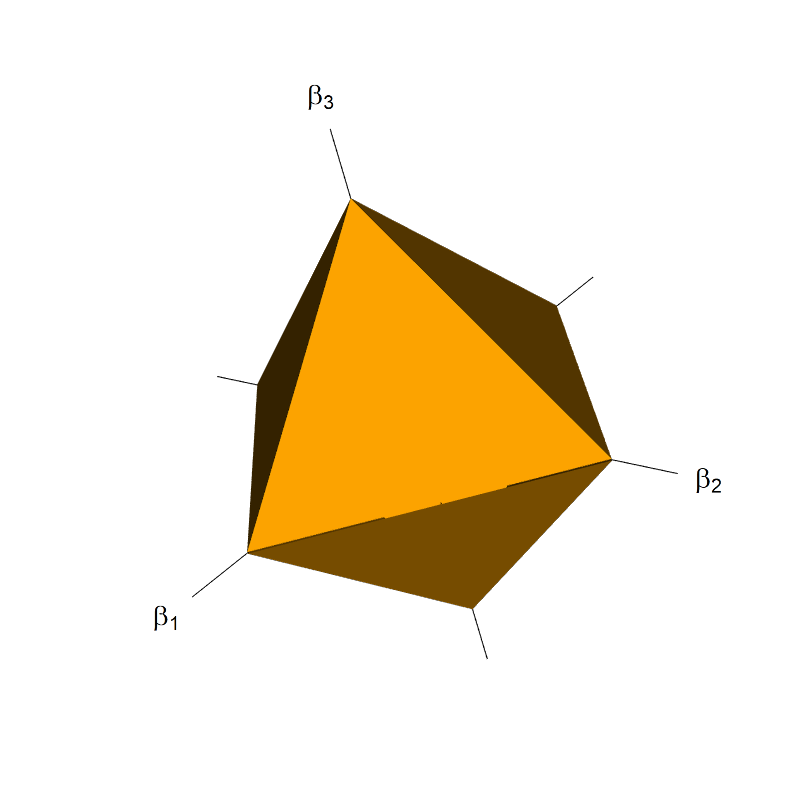
\includegraphics[width = 0.33\textwidth]{3D_lasso_contour.png}
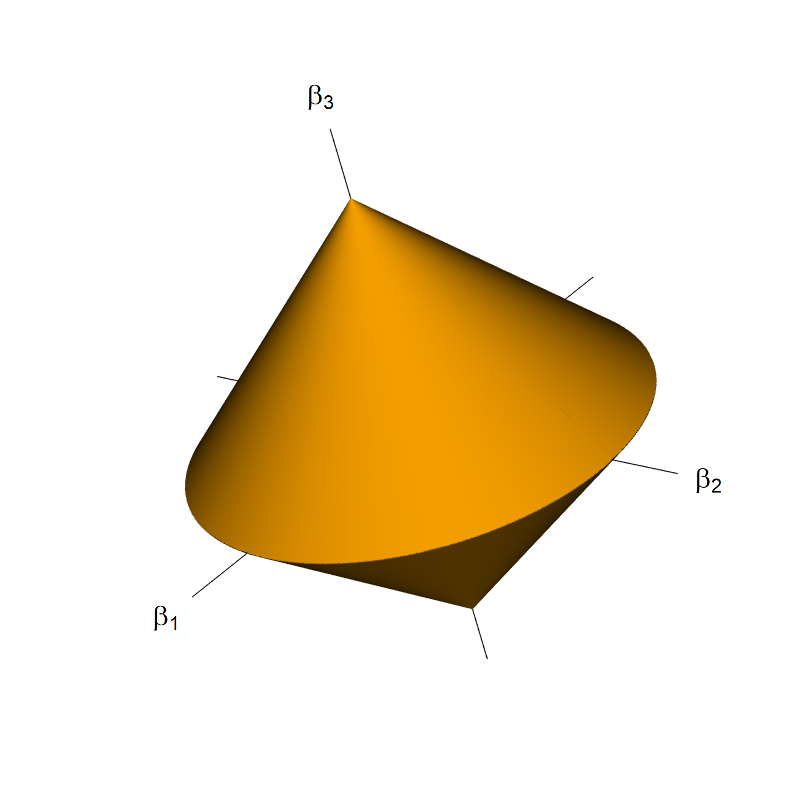
\includegraphics[width = 0.33\textwidth]{3D_glasso_contour.png}
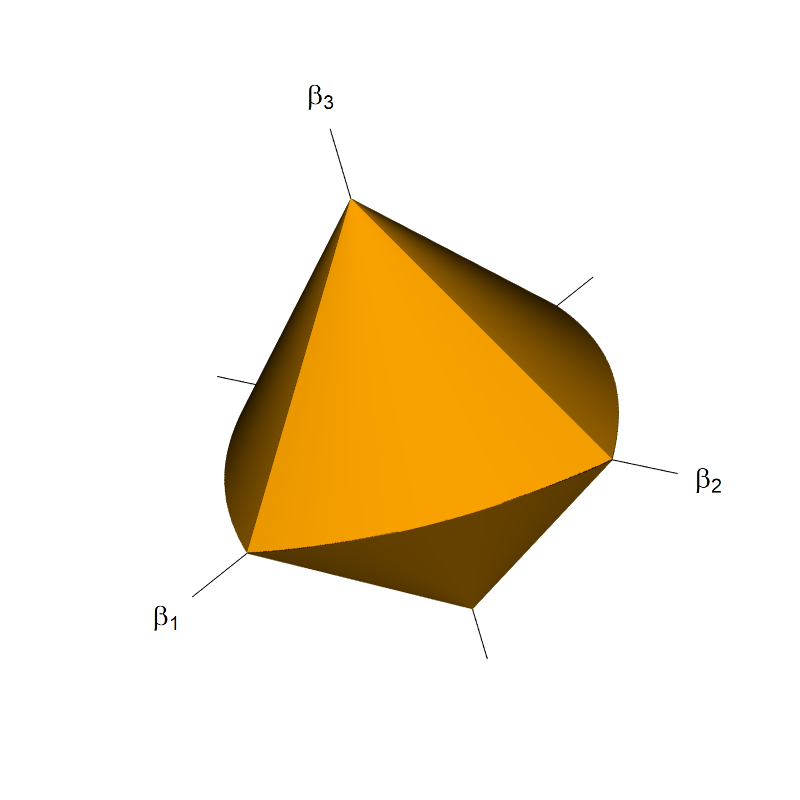
\includegraphics[width = 0.33\textwidth]{3D_sglasso_contour.png}

\caption{Contour lines for the lasso, the gLasso, and the sgLasso for three predictors.}

\end{figure}

\begin{itemize}
    \item In the special case of three predictors, i.e. $\bm{\beta}=(\beta_1,\beta_2,\beta_3)$, the estimated coefficients will lie on the \mydef{contour ball} of the shrinkage penalty. %\pause

    \item In this example, there are two clusters, with $\bm{\beta}_1 = (\beta_1,\beta_2)$ and $\bm{\beta}_2 = \beta_3$. 
    
    \item We can see how within the first cluster, the gLasso imposes an $\ell_2$ penalty, but among different groups it imposes an $\ell_1$ penalty.

    \item For the sgLasso, $\alpha = 0.5$.
    
\end{itemize}   
\end{frame}



\begin{frame}{Sparse Group Lasso}
\begin{itemize}
    \item Sparse Group Lasso differs from Group Lasso because Group Lasso does not provide sparsity of groups and sparsity \emph{within} groups.
    \item Sparse Group Lasso minimizes
    \[
    \min\limits_{\beta} \frac{1}{2n}
    \|\mathbf{y}-\sum\limits_{l=1}\limits^{L} \mathbf{X}_{l}\beta_{l}\|_{2}^{2} +(1-\alpha)\lambda \sum\limits_{l=1}\limits^{L}\sqrt{p_{l}} \|\beta_{l}\|_{2} +
    \alpha \lambda \|\beta\|_{1}
    \]
    \item $\alpha \in [0,1]$ -  a convex combination of the lasso and group lasso penalties
        \begin{enumerate}
            \item $\alpha = 0$ gives group lasso fit
            \item $\alpha = 1$ gives a lasso fit
        \end{enumerate}
    \item Groupwise Sparsity: the number of groups with at least one nonzero coefficient.
    \item Within Group Sparsity: the number of nonzero coefficients within each nonzero group.
    \item Overall Sparsity: the total number of nonzero coefficients irregardless of grouping.
   
\end{itemize}
\end{frame}

\begin{frame}{Sparse Group Lasso}
\begin{itemize}
    \item It looks similar to elastic net penalty, but it is different because $\|.\|_{2}$ is not differentiable at $0$, so some groups are completely zeroed out.
    \item Within each nonzero group it gives an elastic net fit through the $\|.\|_{2}$ penalty parameter a function of the optimal $\|\hat{\beta_{k}}\|_{2}$
    \item $\hat{\beta}$ is the value that minimizes the equation.
    \item On a group sparsity level, group lasso and sparse group lasso act similarly but sparse group lasso adds univariate shrinkage before checking if a group is nonzero.
    \item Sparse group lasso takes into account the likelihood of some levels of predictors being uninformative as the number of levels per predictors increases - sparse group lasso sets the coefficients for many levels to $0$, even in nonzero groups
    \item Sparse group lasso is useful when used on data where the predictors have a natural grouping.
    \item Regarding genomic data, sparse group lasso is useful in finding pathways of interest and selects driving genes from them. 
    \item It shrinks the estimated effects of driving genes within a group toward one another.
\end{itemize}
\end{frame}





\begin{frame}{Principal Component Analysis}

\mydef{Principal component analysis} is a technique for using the principal components of a data set to explain the variance of the data. %\pause
\begin{itemize}
    \item They are a \mydef{linear combination} of the predictors in the data set $\mathbf{X}$. %\pause
\end{itemize}

We will be exploiting their variance-explaining property by using the principal components to help us make predictions. %\pause

The (economy) \mydef{singular value decomposition} (SVD) of a data matrix $\mathbf{X}$ with $m = \mathrm{rank}(\mathbf{X})$ is given by 
\begin{align*}
    \mathbf{X} = \mathbf{U} \mathbf{S} \mathbf{V}^T,
\end{align*} 
where $\mathbf{U}_{n \times m}$ and $\mathbf{V}_{m \times p}$ are orthogonal matrices and $\mathbf{S}_{m \times m}$ is a diagonal matrix. %\pause
\begin{itemize}
    \item The columns of $\mathbf{V}$ are the \mydef{right singular vectors} and the columns of $\mathbf{U}$ are the \mydef{left singular vectors}. %\pause
    \item The \mydef{singular values} of $\mathbf{X}$ are stored in the diagonal of $\mathbf{S}$ in descending order, such that $s_1 \ge \ldots \ge s_m > 0$. %\pause
    \item The columns of $\mathbf{V}$ are the \mydef{principal axes} of $\mathbf{X}$. %\pause
    \item The columns of $\mathbf{US}$ are the \mydef{principal components}.
\end{itemize}
    
\end{frame}

\begin{frame}{The Principal Components Lasso}

\begin{itemize}
    \item PcLasso is suited for data where the number of predictors is much greater than the number of observations.
    
    \item It combines the lasso sparsity penalty with a quadratic penalty that shrinks the coefficient vector towards the leading principal components of the feature matrix.
    
    \item PcLasso exploits the group structure that can exist in a data set.
    
    \item Given pre-existing groups, pcLasso shrinks each group-wise
    component of the solution toward the leading principal components of that group - it also carries out selection of the feature groups. 
    
    \item The objective function is convex - solutions can be found efficiently even for large values of $n$ and $p$.
    
    \item It strongly biases the solution vector toward the leading singular vectors.
\end{itemize}   
\end{frame}

\begin{frame}{Principal Component Lasso}
\begin{itemize}
    \item pcLasso minimizes 
    \[
    \min\limits_{\beta}
    (\frac{1}{2} \| \mathbf{y}-\mathbf{X}\beta\|_2^2 + \frac{\theta}{2}
    \sum\limits_k \beta_k^T
    (\mathbf{V}_k \mathbf{D}_{d^2_{k1}-d^2_{kj}} \mathbf{V}^T_k)\beta_k)
    \]
    \item $\mathbf{X}$ is the $n$ x $p$ matrix ($n$ observations, $p$ predictors)
    
    \item $\beta$ is the vector containing $p$ coefficient estimates.
    
    \item The Singular Value Decomposition of $\mathbf{X=UDV}^{T}$ ($\mathbf{D}$ is a diagonal matrix with diagonal entries consisting of the singular values $d_{1}\geq d_{2}\geq ... \geq d_{m} >0$, where $m=rank(\mathbf{X})$
    
    \item ($\mathbf{V}_k, d_k)$ right singular vectors and singular values of $\mathbf{X}_k$
    
    \item $\beta_k$ is the subvector of $\beta$ corresponding to group $k$
    \item $d_k = (d_{k1},...,d_{km})$ singular values of $\mathbf{X}_k$ in decreasing order.
    \item $\mathbf{D}_{d^2_{k1}-d^2_{kj}}$ diagonal matrix with diagonal entries ${d^2_{k1}-d^2_{kj}}$ for $j=1,2,...,m_k$
    \item The approach to solving this is to fix a few values of $\theta$ and then optimize the equation over a path of $\lambda$ values.
    \item If $\theta = 0$, it becomes equivalent to lasso. 
\end{itemize}
\end{frame}


\begin{frame}{Generalizations}
\begin{itemize}
    \item In the non-group setting, the most general regularization technique, the $\mathbf{Z}$ penalty, is given my \textit{minimizing} the function 
    \begin{align*}
        J = \mathcal{L}(\beta_0, \bm{\beta}) + \lambda \| \bm{\beta} \|_1 + \frac{\theta}{2} \bm{\beta}^T \mathbf{V} \mathbf{Z} \mathbf{V}^T \bm{\beta}.
    \end{align*}
    \item We can see that:
    \begin{enumerate}
        \item This penalty reduces to the \textit{elastic net} when $\mathbf{Z} = \mathbf{I}$.
        \item This penalty reduces to the \textit{pcLasso} when $\mathbf{Z} = \mathbf{D}_{d_1^2 - d_j^2}$.
        \item $\theta = 0$ corresponds to the lasso. 
    \end{enumerate}

    \item In the group lasso, \cite{yuan2006model} consider a more general penalty 
    \begin{align*}
        \mathcal{L}_K(\beta_0, \bm{\beta}) + \lambda \sum_{k=1}^K \sqrt{\bm{\beta}^T \mathbf{R}_k \bm{\beta}}.
    \end{align*}
    \begin{itemize}
        \item Here, $\mathbf{R}_k$ is a penalty matrix for group $k$.
        \item The normal group lasso chooses $\mathbf{R}_1 = \ldots = \mathbf{R}_K = \mathbf{I}$ ( or $\sqrt{p_k} \mathbf{I}$).
        \item The standardized group lasso chooses $\mathbf{R}_k = \mathbf{X}_k^T \mathbf{X}_k$ (have too look into this more). The standardized group lasso was introduced in \cite{simon2012standardization}. In their original paper, the group lasso, the data matrices were designed to be orthogonal, i.e. $\mathbf{X}_k^T = \mathbf{X}_k$ for all $k$. What \texttt{R} packages implement this?
    \end{itemize}
    \item Then the generalization of the sparse group lasso is 
    \begin{align*}
        \mathcal{L}_K(\beta_0, \bm{\beta}) + \lambda \| \bm{\beta} \|_1 + \theta \sum_{k=1}^K \sqrt{\bm{\beta}^T \mathbf{R}_k \bm{\beta}} = \mathcal{L}_K(\beta_0, \bm{\beta}) + \lambda \| \bm{\beta} \|_1 + \theta \sum_{k=1}^K \| \mathbf{R}_k^{1/2} \bm{\beta} \|_2.
    \end{align*}
\end{itemize}
    
\end{frame}





\begin{frame}{Contour Plots}

\begin{figure}
    \centering
    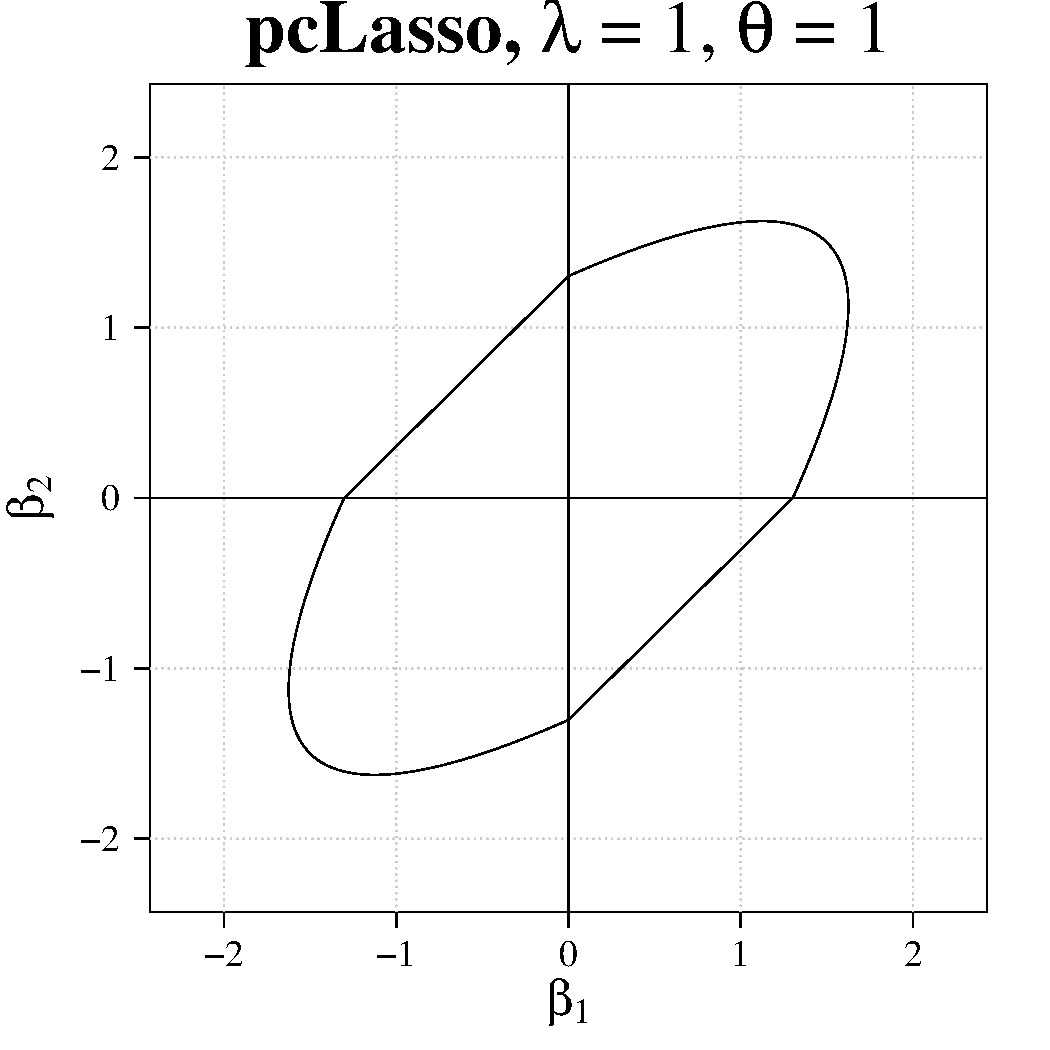
\includegraphics[width = 0.33\textwidth]{Presentation/cont_pcLasso_t3.pdf}
    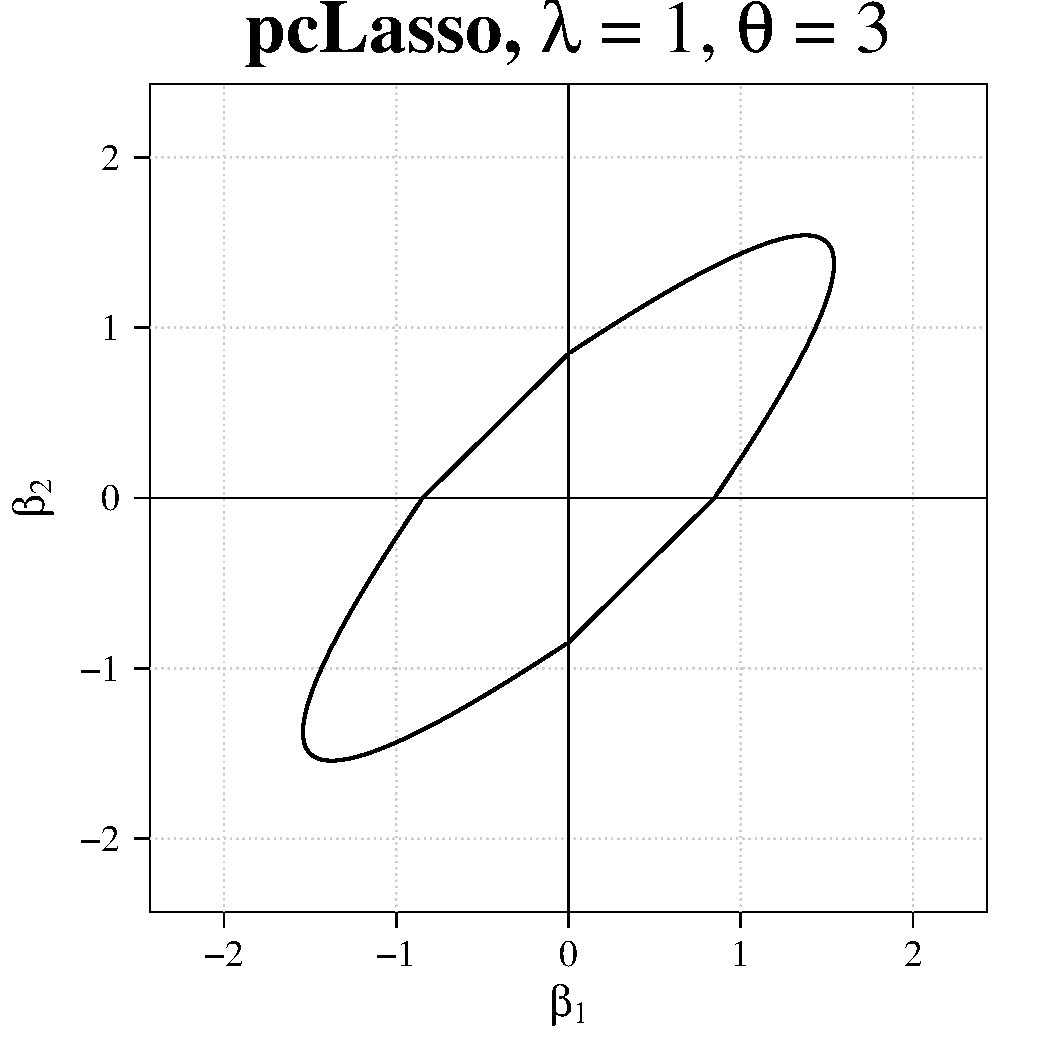
\includegraphics[width = 0.33\textwidth]{Presentation/cont_pcLasso_t2.pdf}
    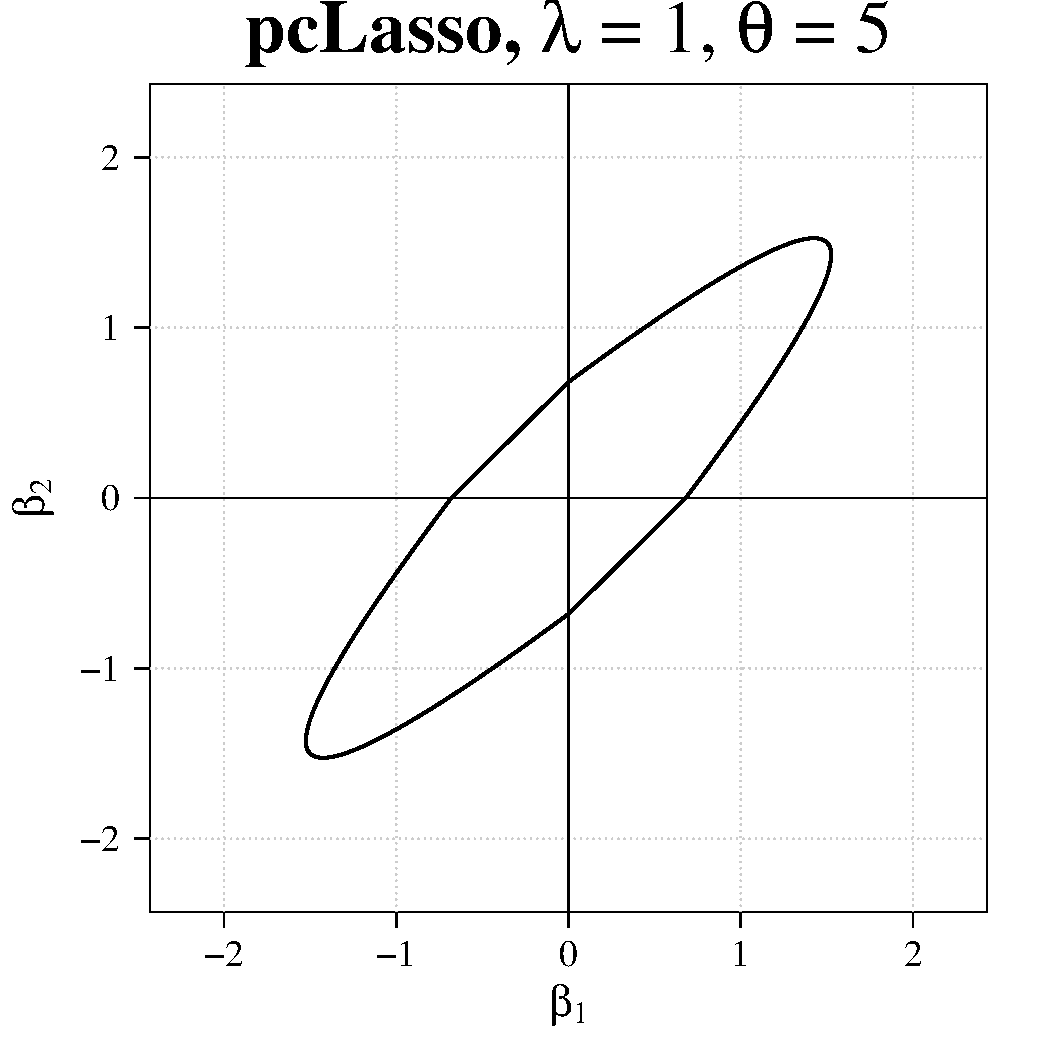
\includegraphics[width = 0.33\textwidth]{Presentation/cont_pcLasso_t1.pdf}
    
    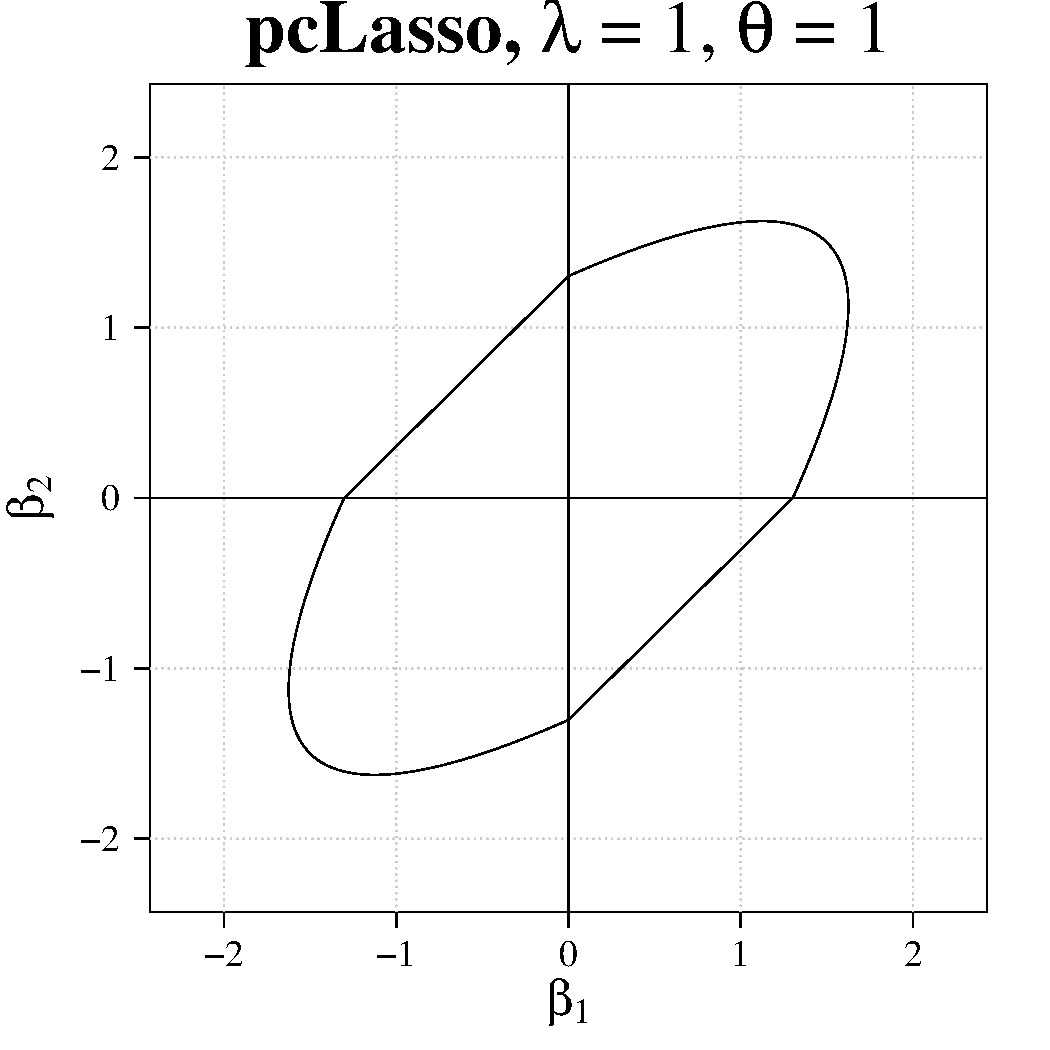
\includegraphics[width = 0.33\textwidth]{Presentation/cont_pcLasso_l3.pdf}
    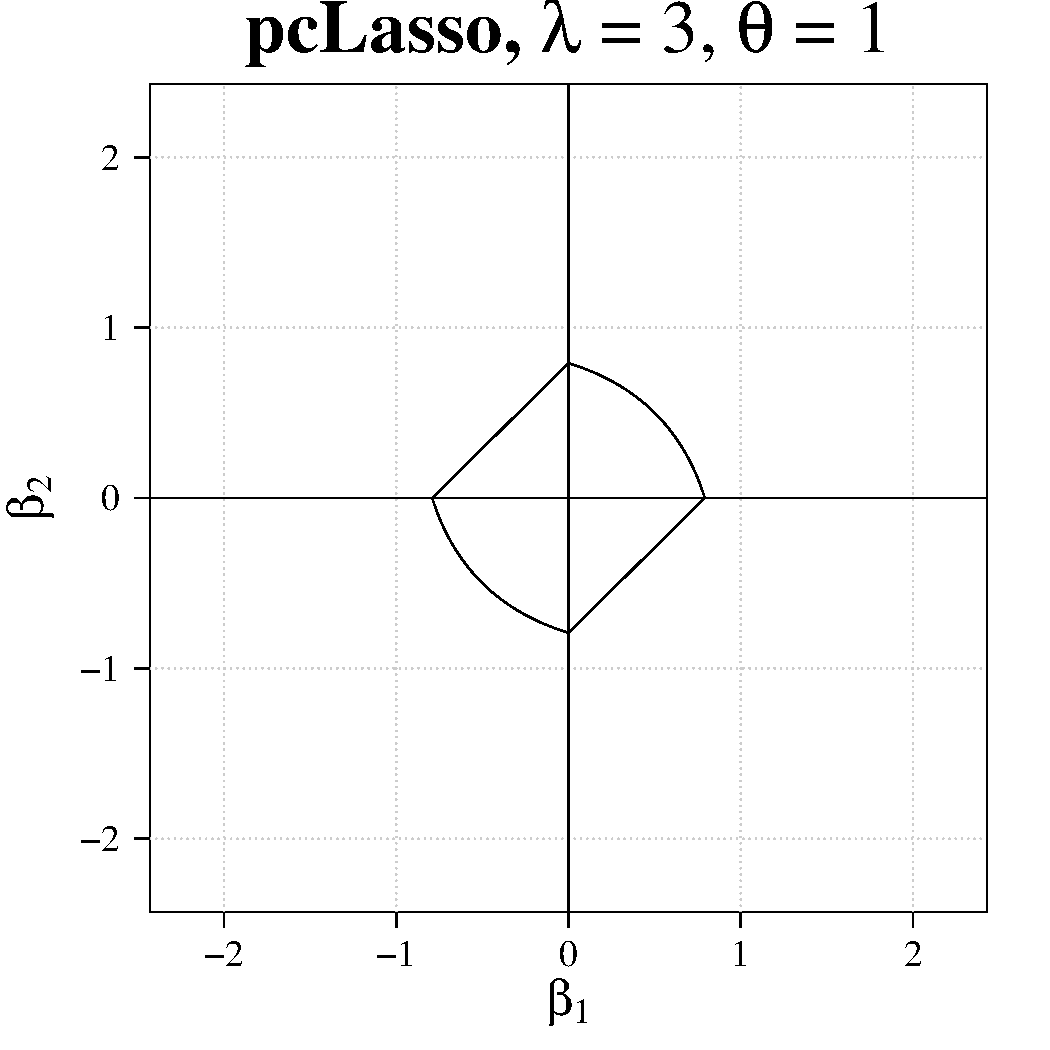
\includegraphics[width = 0.33\textwidth]{Presentation/cont_pcLasso_l2.pdf}
    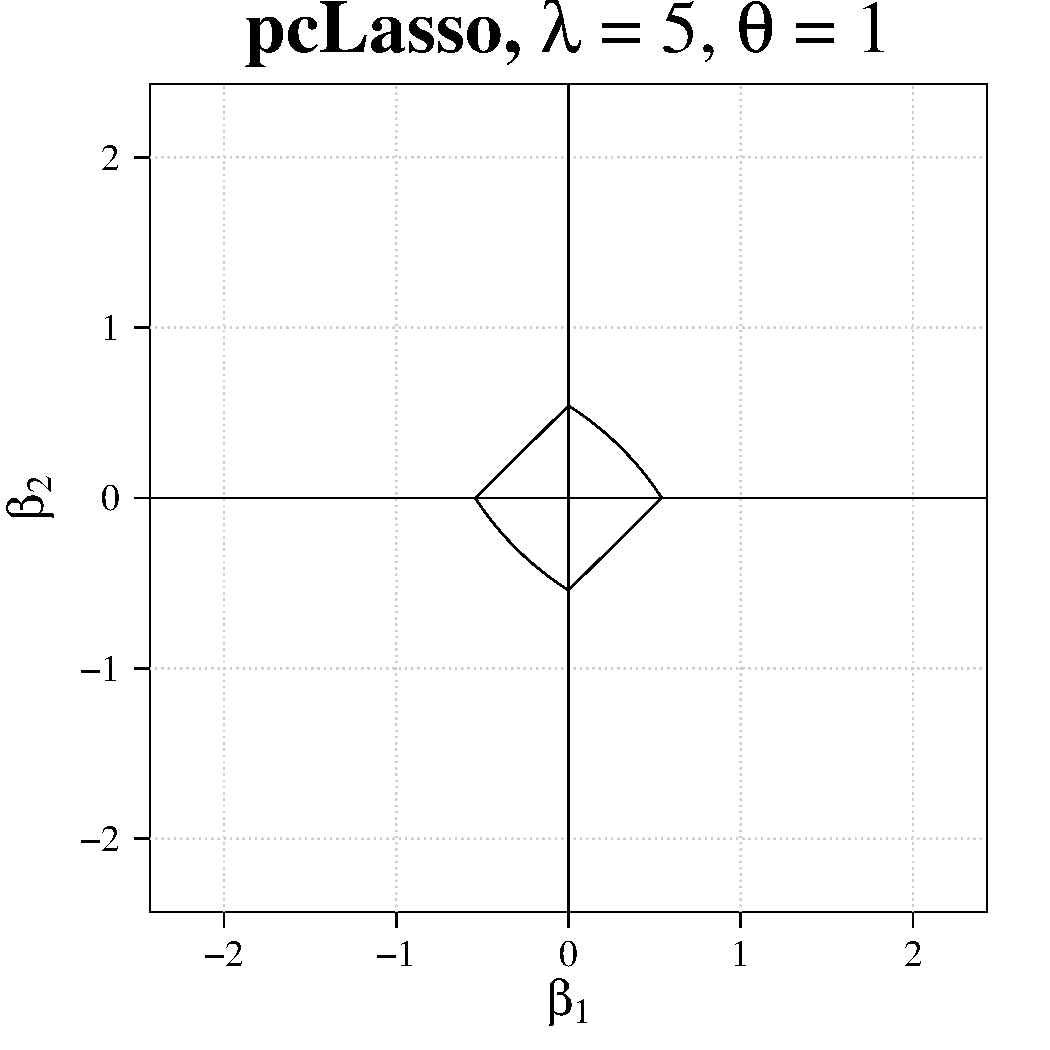
\includegraphics[width = 0.33\textwidth]{Presentation/cont_pcLasso_l1.pdf}
    \caption{Contour plots for pcLasso for various tuning parameters for two predictors.}
    \label{pcLasso_cont}
\end{figure} %\pause
    
\end{frame}









\begin{frame}{Results}

\begin{itemize}

\item Each gene is a variable and in the regression equation, each variable has a coefficient. 
    \item These regularization techniques are used to carry out feature selection of the genes.
    \item Specifically, when lasso is used, some coefficient estimates are pushed to zero.
    \item The number of \textbf{nonzero coefficients} indicate the number of genes (predictors) remain after feature selection is done. These are the influential/significant genes. 
    \item When there is no clustering method used before the regularization technique is applied, each gene is considered individually.
    \item When clustering methods are employed (specifically $K$-means and hierarchical), the predictors are grouped. When the regularization techniques are applied to the clustered data, feature selection occurs on both the group level and the individual level. 
    
\end{itemize}

\end{frame}


\begin{frame}{Results}

\begin{itemize}

    \item When clustering is used, each group has a coefficient as well. The number of \textbf{non-zero groups}  are the number of groups remaining after feature selection is complete. (The groups that were not selected were the ones whose group coefficient became zero)
    \item \textbf{Misclassification} is the amount of error in the model that is produced using the given regularization technique. It gives the proportion of variables that were incorrectly classified by the technique. 
    \item We are trying to see if clustering the data before employing a regularization technique will improve the prediction accuracy of the model.  
    
\end{itemize}
    
\end{frame}



\begin{frame}[allowframebreaks]{References}

\bibliographystyle{apalike}
\bibliography{FPBib}
    
\end{frame}









\end{document}




